\chapter{Conclusions and Discussion}\label{final}
\section{Plots}
\begin{figure}
  \centering
  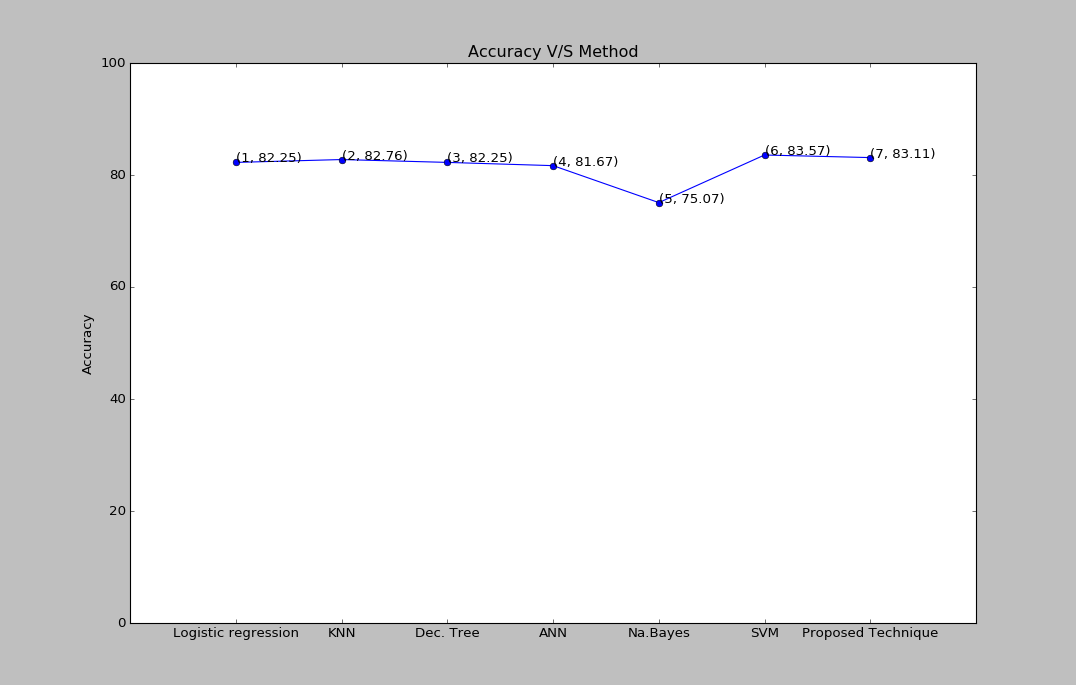
\includegraphics[scale=.45]{i1.png}
  \caption{Accuracies v/s Methods for Data set 1}  
\end{figure}
\begin{figure}
  \centering
  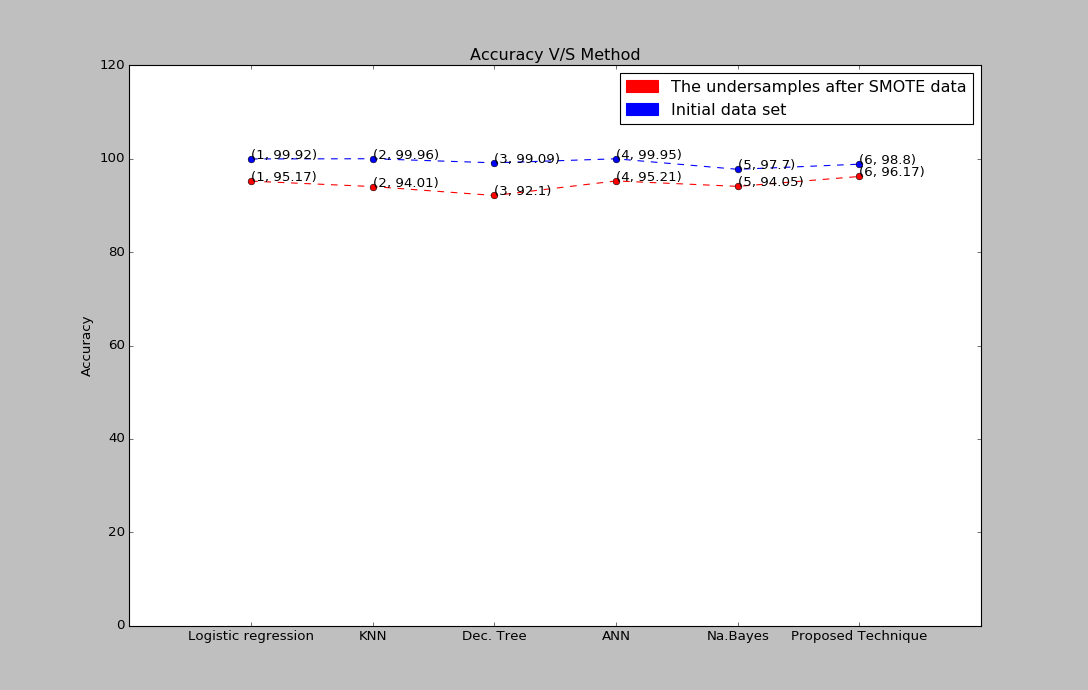
\includegraphics[scale=.45]{i2.png}
  \caption{Accuracies v/s Methos for Dataset 2}
  
\end{figure}
\begin{figure}
  \centering
  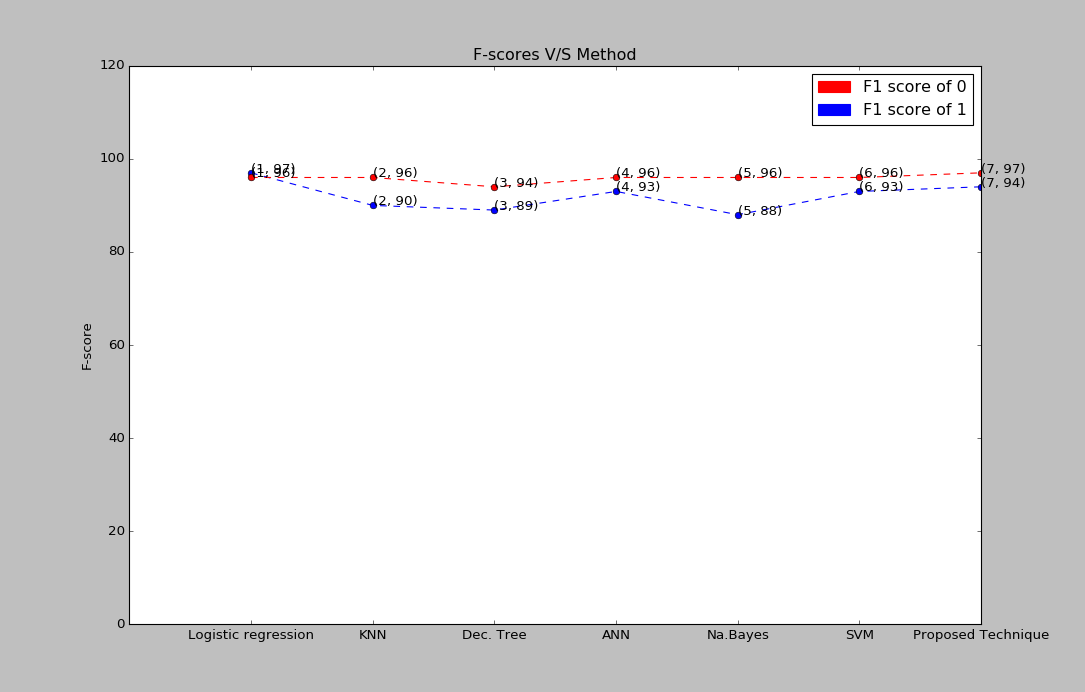
\includegraphics[scale=.45]{i3.png}
  \caption{F1-Scores of 0 and 1 v/s Methods for Dataset 2}
  
\end{figure}

\section{Conclusions}

This report gives rise to a number of important conclusions.
\begin{itemize}
\item In our first data set, we applied all techniques directly to the the given data and found SVM giving us the highest accuracy followed by our proposed methodology. The classification reports among all methods showed very less differences in the accuracies.
\item In the second data set, we applied the techniques before the re-sampling and found our models not predicting the ones properly. Thus some change had to be done in our model. Thus we under-sampled the data and drastically reduced the data set's size to 1300 and then we applied our machine learning techniques.
\item After under-sampling, the overall results were lesser than that of the initial data set but the accuracy and $f1$ score of predicting 1 increased a lot and thus increasing the quality of our models.
\item Again in this data set, our proposed technique of applying K-means with SVM performs slightly better than other techniques.
\item Thus in our report, we applied all machine learning techniques and then compared them to find the best for the data sets.
\end{itemize}

\section{Further Research}
   In our report, we just applied few Machine Learning Techniques and compared. There are many more Advanced Machine Learning Algorithms like Random forests, Boltzmann Algorithms, etc.
   \par In both the data sets, Artificial Neural Networks did not perform very badly. Thus this research work can be extended with the application of Deep Learning Algorithms.
   